\documentclass[12pt]{article}
\usepackage[top=1in,bottom=1in,left=1in,right=1in]{geometry}
\usepackage{alltt}
\usepackage{array}	
\usepackage{graphicx}
\usepackage{tabularx}
\usepackage{verbatim}
\usepackage{setspace}
\usepackage{listings}
\usepackage{amssymb,amsmath, amsthm}

\title{SOEN331: Introduction to Formal Methods\\for Software Engineering\\
Assignment 2 on Extended Finite State Machines}
\author{Martin Marcos 40041398,\\ Samantha Guillemette 26609198,\\ Deepkumar Patel 40096716  }

\date{\today}

\begin{document}
\begin{spacing}{1.5}

\maketitle

\newpage


\section{Driver-less car system formal specification}

\noindent The EFSM of the driver-less car system is the tuple $S = (Q, \Sigma_1, \Sigma_2, q_0, V, \Lambda)$, where\\

\noindent $Q = \{idle, parked~mode, manual~mode, cruise~mode, marked~mode, panic~mode, exit\}$\\
\noindent $\Sigma_1 = \{start~car, cruise~signal, drive~signal, switch, arrived, unforseen,panic,marked~mode~signal, panic~off, engine~off\}$\\
\noindent $\Sigma_2 = \{system~start, engine~idle, beep, system~off, stop~car, hazard~signals~on, hazard~signals~off\}$\\
\noindent $q_0: idle$\\
\noindent $V: nav~system: \{set, not~set, engine~idle, car~stopped\}$\\
\noindent $\Lambda$: Transition specifications\\
\indent 1. $\rightarrow idle$\\
\indent 2. $idle \xrightarrow {\text {start/system start; engine idle}} parked~mode$\\
\indent 3. $parked~mode  \xrightarrow {\text {engine off/system off}} exit$\\
\indent 4. $parked~mode  \xrightarrow {\text {cruise signal[not set]/beep}} manual~mode$\\
\indent 5. $parked~mode  \xrightarrow {\text {cruise signal[set]/beep}} cruise~mode$\\
\indent 6. $parked~mode  \xrightarrow {\text {drive signal[engine idle]}} manual~mode$\\
\indent 7. $manual~mode  \xrightarrow {\text {switch[set]}} cruise~mode$\\
\indent 8. $cruise~mode  \xrightarrow {\text {switch}} manual~mode$\\
\indent 9. $cruise~mode  \xrightarrow {\text {arrived}} parked~mode$\\
\indent 9. $cruise~mode  \xrightarrow {\text {unforseen or panic/stop car; hazard signals on}} panic~mode$\\
\indent 10. $manual~mode  \xrightarrow {\text {marked mode signal[car stopped]}} marked~mode$\\
\indent 11. $panic~mode  \xrightarrow {\text {panic off/hazard signals off}} parked~mode$\\


\noindent The UML state diagram is shown in Figure~\ref{fig:main-system-fig}\\


\noindent The \textit{manual} is a composite state, it is the tuple $S = (Q, \Sigma_1, \Sigma_2, q_0, \Lambda)$, where\\

\noindent $Q = \{running, fast, slower, break~mode\}$\\
\noindent $\Sigma_1 = \{accelerate, decelerate, break\}$\\
\noindent $\Sigma_2 = \{increase~speed, decrease~speed, 0-speed\}$\\
\noindent $q_0: running$\\
\noindent $\Lambda$: Transition specifications\\
\indent 1. $\rightarrow running$\\
\indent 2. $running \xrightarrow {\text { accelerate/increase speed }} faster$\\
\indent 3. $running \xrightarrow {\text { decelerate/decrease speed }} slower$\\
\indent 4. $running \xrightarrow {\text { break/0-speed }} break~mode$\\
\indent 5. $break~mode \xrightarrow {\text { accelerate/increase speed }} running$\\
\indent 6. $faster \xrightarrow {\text { decelerate / decrease speed }} slower$\\
\indent 7. $slower \xrightarrow {\text { decelerate / decrease speed }} slower$\\
\indent 8. $slower \xrightarrow {\text { decelerate / decrease speed }} break~mode$\\

\noindent The UML state diagram is shown in Figure~\ref{fig:manual-mode-fig}\\


\newpage

\section{UML state diagrams}

\begin{figure}[h!]
	\centering
		\includegraphics[width=0.8\textwidth]{./A2_Figures/A2_SOEN331_Main.eps}
		  \caption{Main System.}
  \label{fig:main-system-fig}
\end{figure}

\begin{figure}[h!]
	\centering
		\includegraphics[width=0.8\textwidth]{./A2_Figures/A2_SOEN331_Manual.eps}
		  \caption{Manual Mode.}
  \label{fig:manual-mode-fig}
\end{figure}

\end{spacing}

\end{document}
